\chapter*{Questão 4}
% Enunciado
\noindent {\it Seja o sistema da Fig. \ref{fig:q4:sist}. Considerando $G(s) =
\frac{2e^{-s}}{s+0.25}$, pede-se: }

\begin{itemize}
    \item[a)] {\it projetar um controlador PI de forma que o desempenho do
              sistema em malha fechada não apresente sobre-sinal. Simule a 
              resposta no Matlab.}
    \item[b)] {\it Considerando o sistema com o controlador projetado no item a
              e considerando $G_d(s) = 1$, projetar um controlador feedforward 
              (realizável) e avaliar o desempenho do sistema completo utilizando
              o Matlab.}
\end{itemize}

\begin{figure}[H]
\centering
    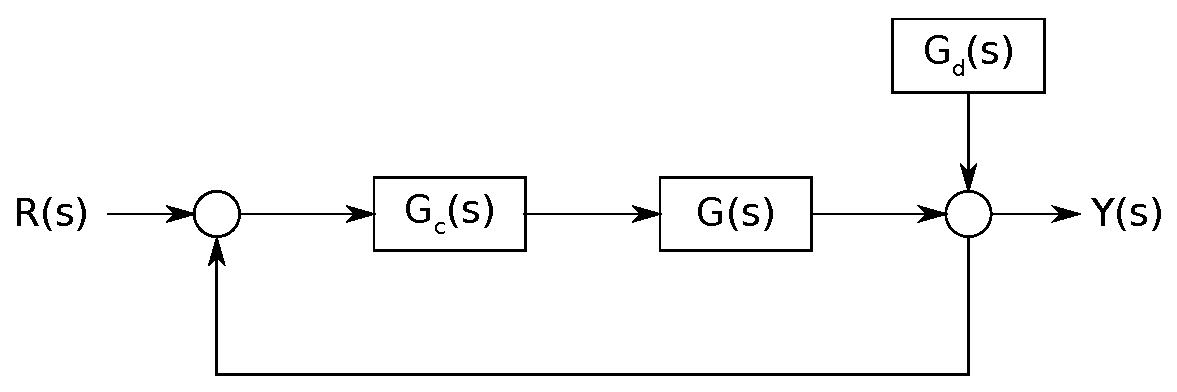
\includegraphics[width=0.65\textwidth]{imgs/questao4/sistema}
    \caption{Diagrama de blocos do sistema.}
    \label{fig:q4:sist}
\end{figure}

\vspace{0.5cm}

\noindent{\bf Resolução:}

\vspace{0.25cm}

O controlador PI foi projetado utilizando o método tradicional, ou seja,
desconsiderando o atraso do sistema, ou seja, separando o termo $e^{-s}$ do
restante da função de transferência, como pode ser visto na figura
\ref{fig:q4:projetoPI}. Definimos então $G'(s)$, como sendo a função de
transferência sem o atraso de transporte, ou seja:

\begin{flalign*}
G'(s) = \frac{2}{s+0.25}
\end{flalign*}

\begin{figure}[htb]
\centering
\scalebox{0.7}{\begin{picture}(0,0)%
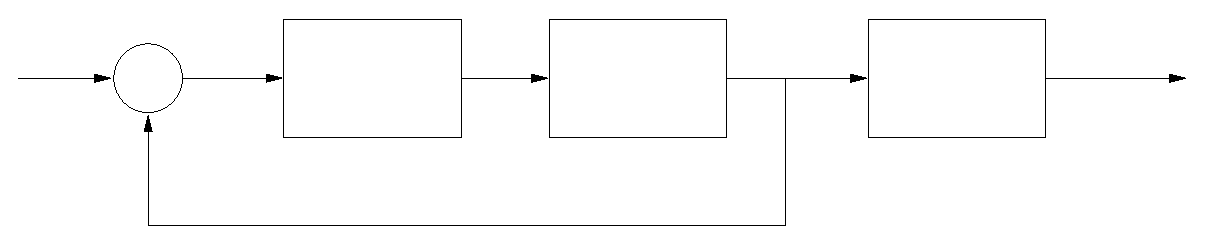
\includegraphics{./imgs/questao4/projetoPI.eps}%
\end{picture}%
\setlength{\unitlength}{4144sp}%
%
\begingroup\makeatletter\ifx\SetFigFont\undefined%
\gdef\SetFigFont#1#2#3#4#5{%
  \reset@font\fontsize{#1}{#2pt}%
  \fontfamily{#3}\fontseries{#4}\fontshape{#5}%
  \selectfont}%
\fi\endgroup%
\begin{picture}(8934,1599)(2914,-3448)
\put(3241,-2176){\makebox(0,0)[b]{\smash{{\SetFigFont{12}{14.4}{\familydefault}{\mddefault}{\updefault}{\color[rgb]{0,0,0}$R(s)$}%
}}}}
\put(5626,-2356){\makebox(0,0)[b]{\smash{{\SetFigFont{12}{14.4}{\familydefault}{\mddefault}{\updefault}{\color[rgb]{0,0,0}$G_c(s)$}%
}}}}
\put(3511,-2536){\makebox(0,0)[b]{\smash{{\SetFigFont{12}{14.4}{\familydefault}{\mddefault}{\updefault}{\color[rgb]{0,0,0}$+$}%
}}}}
\put(4096,-2716){\makebox(0,0)[b]{\smash{{\SetFigFont{12}{14.4}{\familydefault}{\mddefault}{\updefault}{\color[rgb]{0,0,0}$-$}%
}}}}
\put(7651,-2356){\makebox(0,0)[b]{\smash{{\SetFigFont{12}{14.4}{\familydefault}{\mddefault}{\updefault}{\color[rgb]{0,0,0}$\frac{2}{s+0.25}$}%
}}}}
\put(10081,-2356){\makebox(0,0)[b]{\smash{{\SetFigFont{12}{14.4}{\familydefault}{\mddefault}{\updefault}{\color[rgb]{0,0,0}$e^{-s}$}%
}}}}
\put(8911,-2131){\makebox(0,0)[b]{\smash{{\SetFigFont{12}{14.4}{\familydefault}{\mddefault}{\updefault}{\color[rgb]{0,0,0}$Y'(s)$}%
}}}}
\put(11341,-2131){\makebox(0,0)[b]{\smash{{\SetFigFont{12}{14.4}{\familydefault}{\mddefault}{\updefault}{\color[rgb]{0,0,0}$Y(s)$}%
}}}}
\end{picture}%
}
\caption{Projeto de controlador desconsiderando o atraso de transporte.}
\label{fig:q4:projetoPI}
\end{figure}

Primeiramente, analisou-se o sistema em malha fechada do sistema dado o
comportamento sem nenhum controlador ou seja $G_c(s) = 1$. O
comportamento pode ser tomando como aceitável já que se aproxima do erro de
regime nulo e tem um tempo de subida razoável (menos de $1$s) (ver figura
\ref{fig:q4:saida_mf}). Com o controlador PI está adequadamente empregado já
que tem o objetivo de melhorar o erro de regime.

\begin{figure}[htb]
\centering
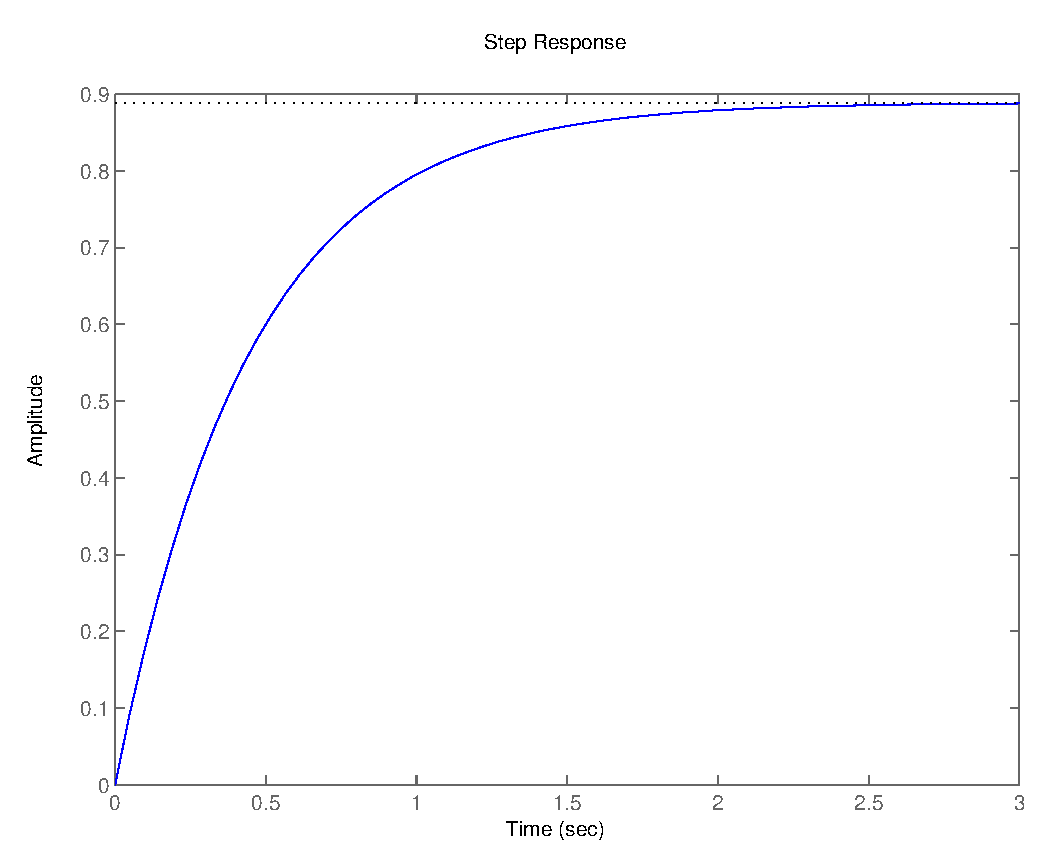
\includegraphics[width=0.65\textwidth]{imgs/questao4/saida_mf}
\caption{Saída do sistema sem o controlador}
\label{fig:q4:saida_mf}
\end{figure}

O requisito do sistema projetado foi a não-presença do sobre-sinal
(\emph{overshoot}). Dessa forma os polos de $G_c(s)G'(s)$ não deviam se afastar
do eixo real, o que significaria oscilações no sinal de saída. O controlador PI
\cite{Araujo} tem a seguinte função de transferência:

\begin{flalign*}
G_c(s) = k_p + \frac{k_i}{s} = \frac{k_c(s+z)}{s}
\end{flalign*}

Logo o controlador adiciona um polo na origem e um zero. Para não afetar
demasiadamente as características do transitório, decidimos posicionar o zero do
controlador antes do polo do sistema $G'(s) = \frac{2}{s + 0.25}$, ou seja $|z|
< 0.25$. Foi simulador então a resposta do sistema com o seguinte controlador
desenvolvido

\begin{flalign*}
G_c(s) = \frac{s+0.2)}{s}
\end{flalign*}

\noindent e os resultados obtidos na simulação podem ser visualizados na figura
\ref{fig:q4:saida_comp_mf}. O diagrama do lugar das raízes para o sistema com o
controlador pode também ser visualizado na figura \ref{fig:q4:rlocus_cmf}.

\begin{figure}[htb]
\centering
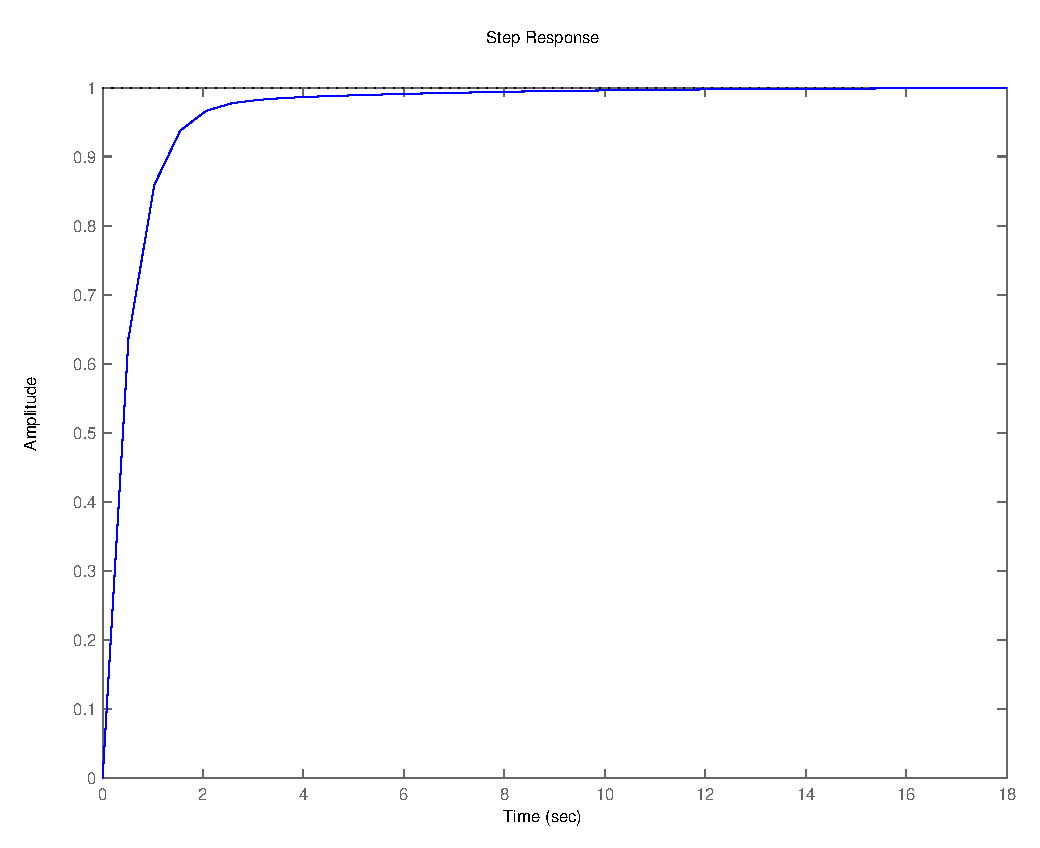
\includegraphics[width=0.65\textwidth]{imgs/questao4/saida_comp_mf}
\caption{Saída do sistema com o controlador projetado $G_c(s) =
\frac{s+0.2}{s}$}
\label{fig:q4:saida_comp_mf}
\end{figure}

% TODO(crisgc): Melhorar a figura no matlab
\begin{figure}[htb]
\centering
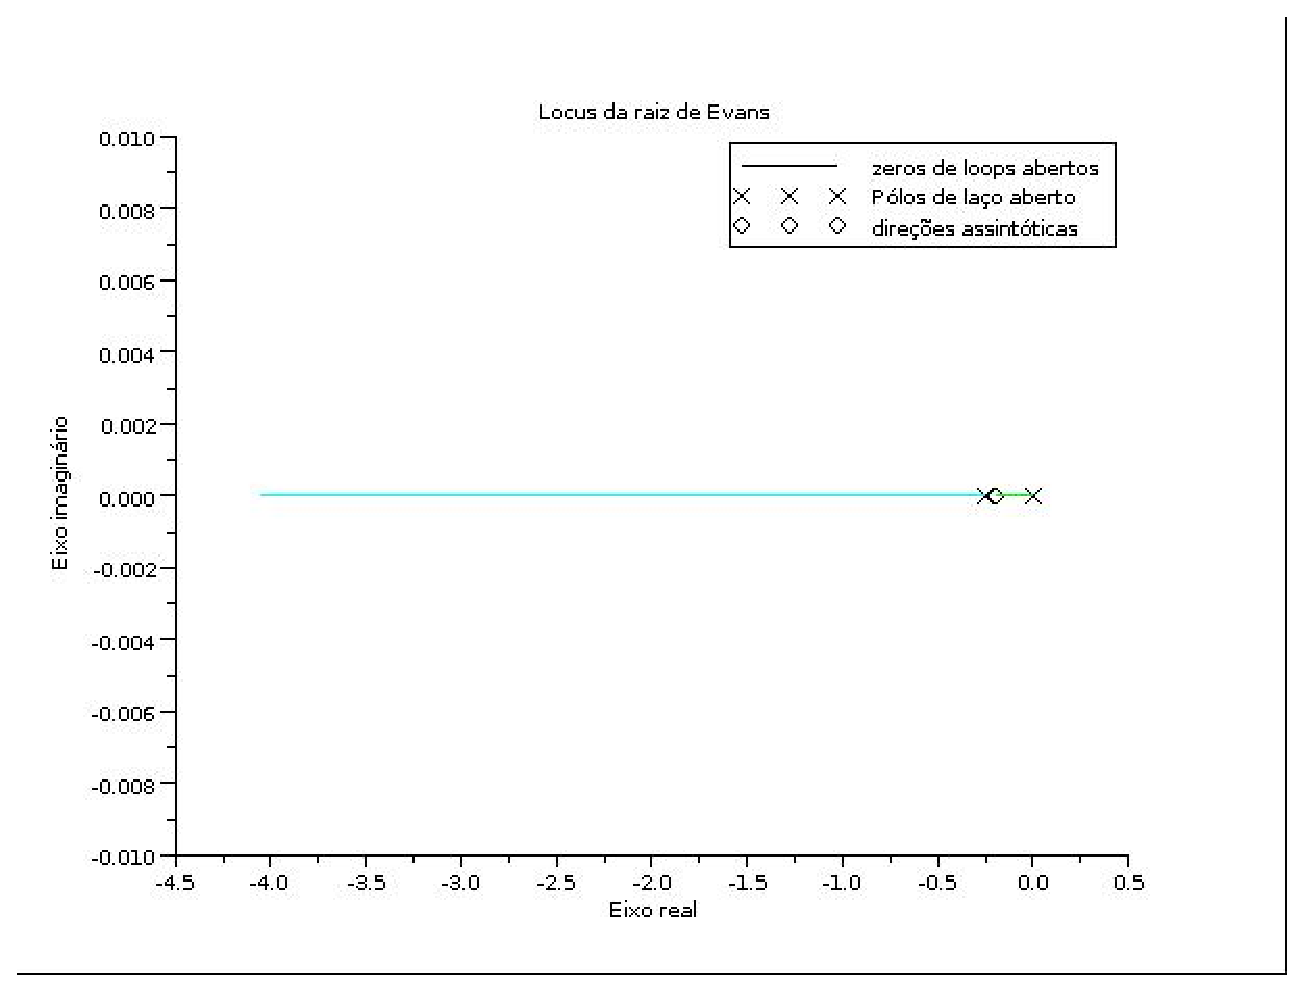
\includegraphics[width=0.65\textwidth]{imgs/questao4/rlocus_cmf}
\caption{Lugar das raízes para $G_c(s)G'(s) = \frac{0.4+2s}{0.25s+s^{2}}$}
\label{fig:q4:rlocus_cmf}
\end{figure}

A função de transferência de malha fechada para do sistema com o controlador,
juntamente com o valor de $\omega_n$ e $\zeta$ é portanto:

\begin{flalign*}
G'_{\text{MF}}(s) & = \frac{G_c(s)G'(s)}{1+G_c(s)G'(s)} =
\frac{0.4+2s}{0.4+2.25s+s^{2}} \\
\omega_n & \approx 0.632 \\
\zeta & \approx 1.779
\end{flalign*}

Percebe-se que o sistema é sobreamortecido, já que $\zeta > 1$ \cite{Medeiros},
portanto a resposta não apresenta o sobressinal. Simulou-se então através de
\Simulink\ o desempenho do compensador PI projetado no controle do sistema
$G(s)$ original, ou seja, com o atraso de transporte. O desempenho foi
completamente insatisfatório: o sistema tornou-se instável (ver figura . 

\begin{figure}[htb]
\centering
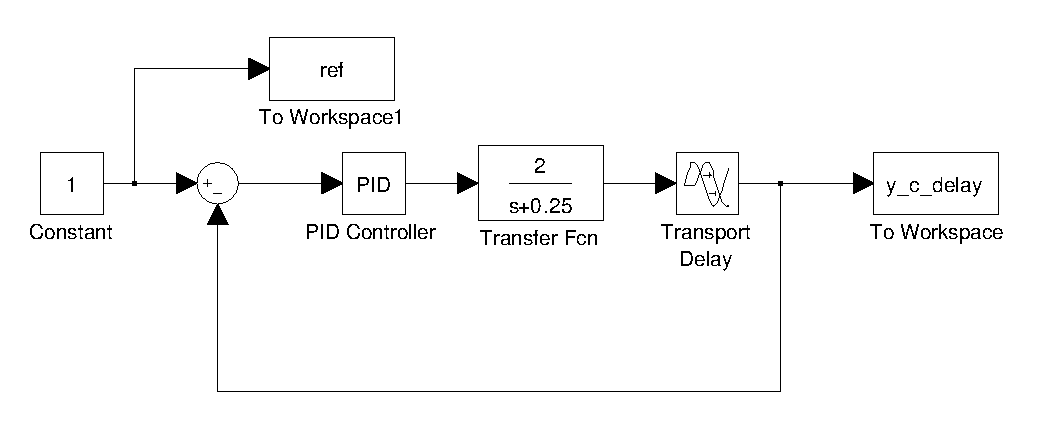
\includegraphics[width=0.65\textwidth]{imgs/questao4/sist_cont_dt}
\caption{Sistema com atraso controlado pelo PI}
\label{fig:q4:sist_cont_dt}
\end{figure}

\begin{figure}[htb]
\centering
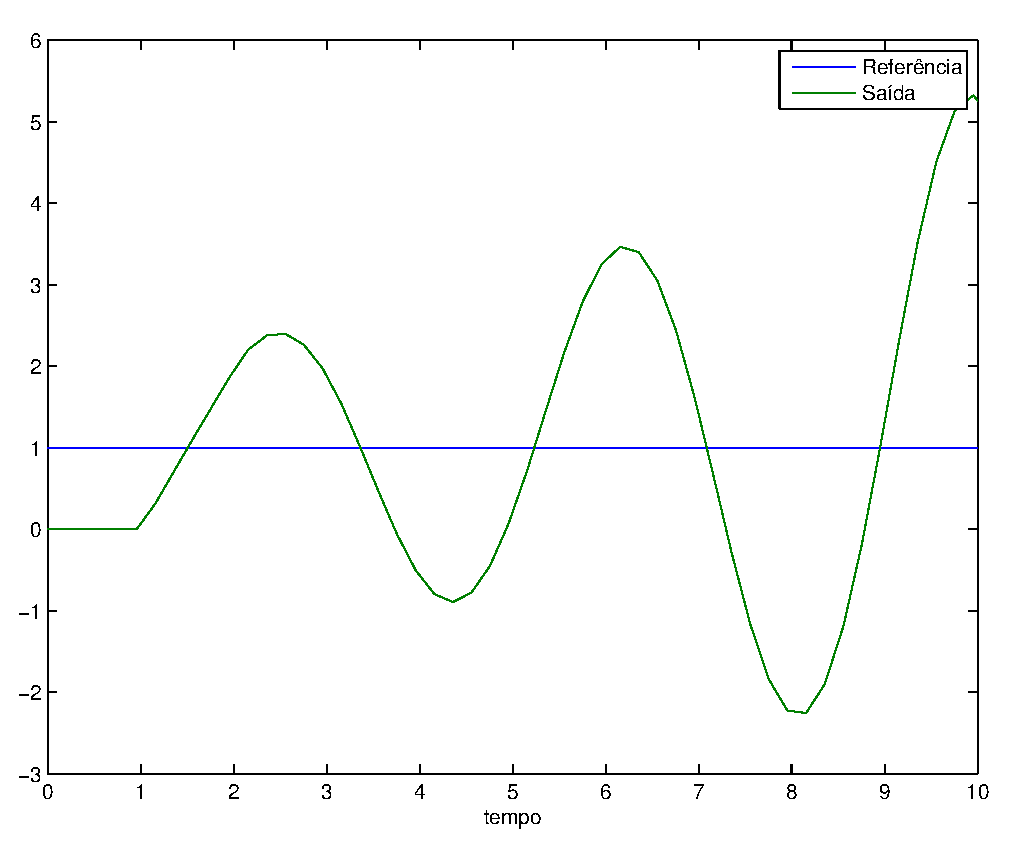
\includegraphics[width=0.65\textwidth]{imgs/questao4/saida_cont_dt}
\caption{Resposta do sistema da figura \ref{fig:q4:sist_cont_dt}}
\label{fig:q4:saida_cont_dt}
\end{figure}

Foi adotado então o preditor de Smith, esse tipo de arquitetura implementa um tipo
de predição baseado no modelo e possibilita ao controlador projetado agir
baseado na predição $y'(t + L)$, onde $L$ é o tempo morto, ou em outras
palavras, o preditor   \cite{Haegglund1996}. \citeasnoun{Haegglund1996}
também justifica porque o tipo de controlador normalmente usado com preditor de
Smith é o PI e explica porque Ele melhora o desempenho já que 
